% This is auto-generated file: do not edit!
% Exported from microMathematics Plus, version 2.23.2


Este ejemplo muestra gráficos en 3D
para tres funciones diferentes de dos
variables.

Primero, definimos los intervalos para
los argumentos x e y. El intervalo
para el eje x depende del número de
puntos a lo largo del eje x y de los
valores mínimo y máximo, x1 y x2:
\begin{center}\begin{tabular}{ccc}
  $N := 300$ &
  $x1 := -2$ &
  $x2 := 2$ \cr
\end{tabular}\end{center}
\begin{center}\begin{tabular}{c}
  $x := \left[ x1,\, x1 +  \left| x2 - x1 \right|  / N \,..\, x2 \right]$
\end{tabular}\end{center}

El intervalo para el eje y está
definido análogamente:
\begin{center}\begin{tabular}{ccc}
  $M := 300$ &
  $y1 := -3$ &
  $y2 := 3$ \cr
\end{tabular}\end{center}
\begin{center}\begin{tabular}{c}
  $y := \left[ y1,\, y1 +  \left| y2 - y1 \right|  / M \,..\, y2 \right]$
\end{tabular}\end{center}

Por ejemplo, trazaremos una función
trigonométrica que es un producto del
seno y el coseno:
\begin{center}\begin{tabular}{c}
  $F(x,y) := sin \left( 3 \cdot {x}^{2}\right)  \cdot cos \left( {y}^{2}\right) $
\end{tabular}\end{center}

Para crear una vista en 3D, haga clic
en el botón ''Nuevo elemento'' de la
barra de acciones o en el botón
''Añadir gráfico 3D'' de la barra de
herramientas:
\begin{center}\begin{tabular}{c} 
\includegraphics[width=0.45\textwidth]{graphics/three_d_plot_fig1.png} \end{tabular}\end{center}

Coloca el nombre de la función F(x,y)
en el campo central-inferior:
\begin{center}\begin{tabular}{c} 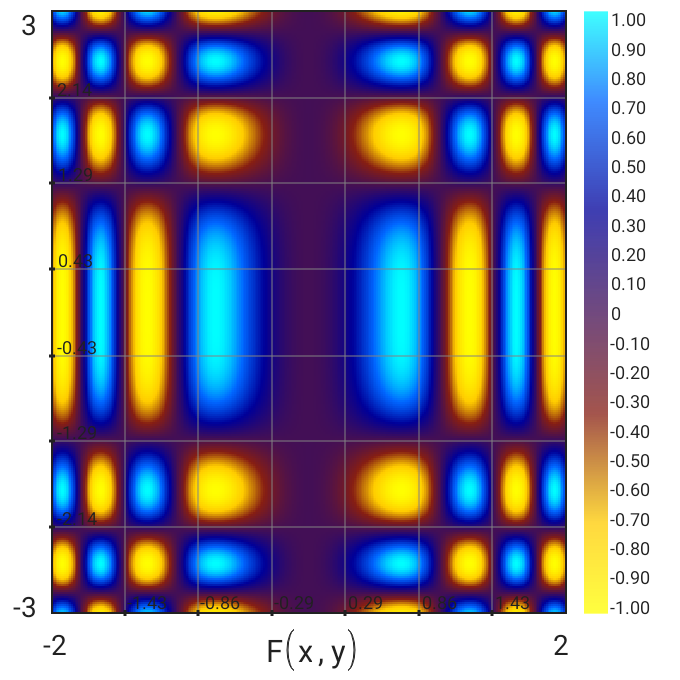
\includegraphics[width=0.45\textwidth]{graphics/three_d_plot_fig2.png} \end{tabular}\end{center}

Los límites del gráfico, el tamaño y el
estilo de los trazos, las etiquetas y
la cuadrícula se pueden ajustar por
analogía con el gráfico de funciones
utilizando el diálogo de ajustes de
gráficos (véase el ejemplo ''Gráfico de
la función'' de la caja de navegación
de aplicaciones para obtener más
detalles). Para abrir este cuadro de
diálogo, mantén presionado en el área
del gráfico hasta que aparezca el
botón flotante ''Propiedades del
objeto'', y luego pulse en este botón.

Adicionalmente, puede cambiar el
número de etiquetas a lo largo del eje
z y elegir la paleta de colores en el
cuadro de diálogo ''Ajustes de color de
la tabla''. Este diálogo aparece al
mantener presionado en la barra del
eje z a la derecha del área del
gráfico principal.
\begin{center}\begin{tabular}{c}
  $R(x,y) := sin \left( 5 \cdot {x}^{2} \cdot \left( y - x \right)\right) $
\end{tabular}\end{center}
\begin{center}\begin{tabular}{c} 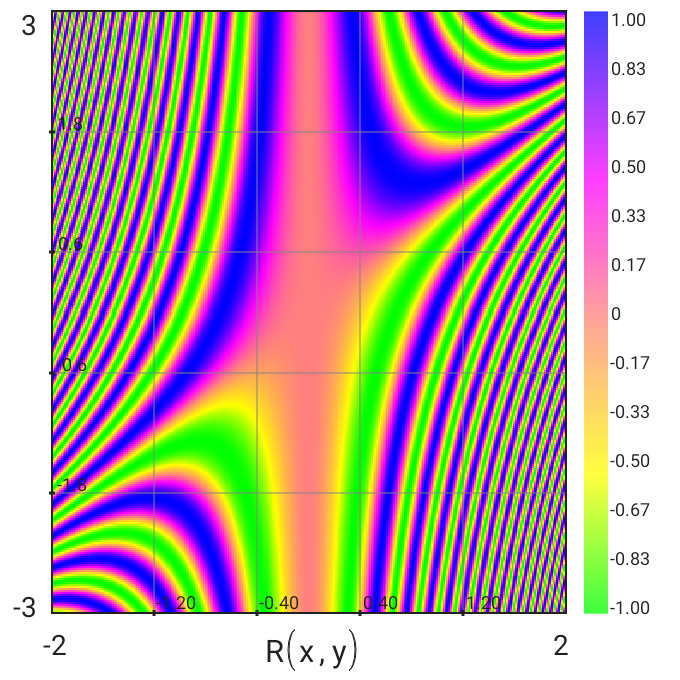
\includegraphics[width=0.45\textwidth]{graphics/three_d_plot_fig3.png} \end{tabular}\end{center}

También se puede trazar una función de
dos argumentos como una superficie en
el espacio 3D. Este modo puede
activarse en el cuadro de diálogo
''Ajustes de la gráfica'' que aparece si
se pulsa en el botón flotante
''Propiedades del objeto'' después de
hacer un largo pulso en el área del
trazado. Trazamos la siguiente
función, utilizando matrices para
mejorar el tiempo de cálculo:
\begin{center}\begin{tabular}{cccc}
  $N := 100$ &
  $n := \left[ 0,\, 1 \,..\, N \right]$ &
  $x1 := -15$ &
  $x2 := 15$ \cr
\end{tabular}\end{center}
\begin{center}\begin{tabular}{cccc}
  $M := 100$ &
  $m := \left[ 0,\, 1 \,..\, M \right]$ &
  $y1 := -15$ &
  $y2 := 15$ \cr
\end{tabular}\end{center}
\begin{center}\begin{tabular}{c}
  $x_{n}  := {\left( x1 +  \left( x2 - x1\right)  \cdot n / N \right)}^{2}$
\end{tabular}\end{center}
\begin{center}\begin{tabular}{c}
  $y_{m}  := {\left( y1 +  \left( y2 - y1\right)  \cdot m / M \right)}^{2}$
\end{tabular}\end{center}
\begin{center}\begin{tabular}{c}
  $r_{n,\, m}  := 0.04 \cdot x_{n}  + 0.02 \cdot y_{m} $
\end{tabular}\end{center}
\begin{center}\begin{tabular}{c}
  $t_{n,\, m}  := \left( x_{n}  + 0.05 \cdot y_{m}  \right) \cdot exp \left( 1 - r_{n,\, m} \right) $
\end{tabular}\end{center}
\begin{center}\begin{tabular}{c}
  $F_{n,\, m}  := \frac{sin \left( x_{n}  + 0.1 \cdot y_{m} \right) }{0.15 + r_{n,\, m} } + \frac{t_{n,\, m} }{10}$
\end{tabular}\end{center}
\begin{center}\begin{tabular}{c} 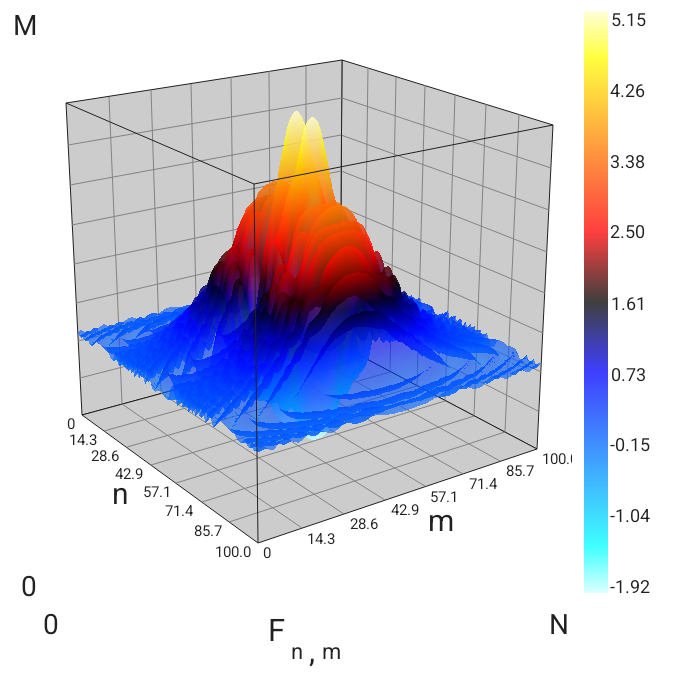
\includegraphics[width=0.45\textwidth]{graphics/three_d_plot_fig4.png} \end{tabular}\end{center}

Para el gráfico de la superficie, hay
ajustes adicionales presentados en el
diálogo ''Ajustes de la gráfica''.
Puedes elegir si se muestran las
líneas de malla, seleccionar la
opacidad para el color de la malla,
definir los ángulos de rotación y
elevación del cuadro de trazado. Por
ejemplo, la superficie anterior
trazada con otros ángulos de rotación
y elevación se ve así: 
\begin{center}\begin{tabular}{c} 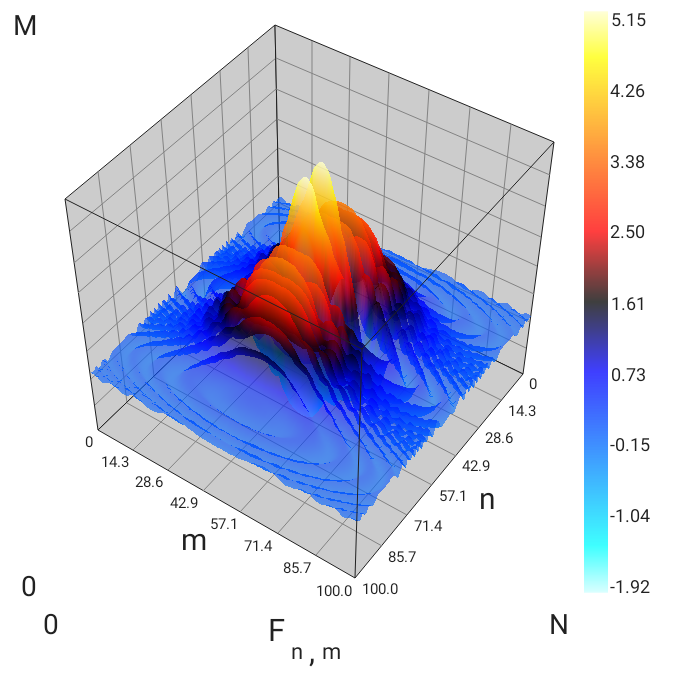
\includegraphics[width=0.45\textwidth]{graphics/three_d_plot_fig5.png} \end{tabular}\end{center}